%!TEX root = ../main.tex
%% Chapter 3 - Benchmark


\chapter{Benchmark}
In computer science, a benchmark is an act of running a program that will put the machine under stress situation, in order to measure the performance. 
Several types of benchmarks exist in order to evaluate the performance of individual components of a machine. 
In the context of this bachelor work, a database benchmark has been run in order to evaluate the performance of OpenStack.
This section presents the tools and the benchmark used.

%%--------------- subsection
\section{TPC-C benchmark}
For our experiments, we used the TPC-C benchmark. 
TPC-C is defined as an \enquote{\textit{on-line transaction processing (OLTP) benchmark}}\footnote{\url{http://www.tpc.org/tpcc}, 14.09.2014} by the Transaction Processing Performance Council (TPC).
The performance of a given system is measured by simulating an OLTP database environment in which concurrent transactions happen.
Thus, a typical OLTP application depicting a wholesale supplier is used 
and only activities or tasks having an impact on resource utilization are considered, as they may affect the performance of the whole system.
This means that activities requiring small resource utilization and/or appearing with low frequency are completely ignored, 
letting just the most significant ones (Table \ref{table:tpcc_trans_type_list}) to evaluate the performance.
To better understand how this benchmark evaluates a system, one must understand how the chosen wholesale supplier is organized.
In this environment, we have a hierarchy. 
Beginning at the top, we have the company, which has several warehouses in different places, each one having 100000 items in stock.
Ten sales districts are distributed around each warehouse.
Each one of these sales districts serves 3000 clients (or customers).
The company receives new orders (composed of 5 up to 15 order lines) from clients.
The clients also have the possibility to check the statuses of their orders by contacting the company.
Among all the order lines, 1\% are for items that are not in-stock at a given warehouse.
These items have to be provided by another warehouse.
Finally, the company has to deal with clients' payments, order processing and stock levels.
Of course, as the business is growing, new warehouses and everything that comes after will be created.

\begin{table}[h]
	\centering
	\begin{tabular}{|m{4cm}|m{9cm}|}
		\hline
		\textbf{Transaction type} & \textbf{Description}\\
		\hline
		New Order & enters a new order into the database\\
		\hline
		Payment & updates the customer balance\\
		\hline
		Order Status & checks the status of an order\\
		\hline
		Delivery & processes batch of new orders not yet delivered\\
		\hline
		Stock Level & determines the number of sold items that have a low stock level (depending on threshold)\\
		\hline
	\end{tabular}
	\caption{TPC-C Transaction Types}
	\label{table:tpcc_trans_type_list}
\end{table}

From this system description, one can see that it has to deal with a lot of transactions, especially if the number of warehouses increases.
The corresponding TPC-C database, consisting of nine tables, is depicted by the entity-relationship diagram shown in Figure \ref{fig:tpcc_erd}.
One can see that the number of warehouses is the scale factor of this database, meaning that the more warehouses there are, the bigger the size of the database will be.
Indeed, the number of rows in each table is a function of the given number of warehouses.
The table ``Item'' is an exception and has a fixed number of rows.

\begin{figure}[h]
	\centering
	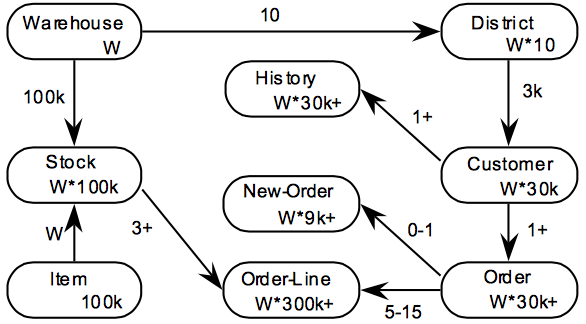
\includegraphics[scale=0.5]{figures/tpcc_erd.png}
	\caption{TPC-C database ER diagram \cite[p. 11]{tpcc10}}
	\label{fig:tpcc_erd}
\end{figure}

During a benchmark run, simulated users are interacting with the system by issuing different transactions, which are then processed by TPC-C.
It returns the performance in the number of transactions per minute C (tpmC, the letter \textit{C} denotes the type of benchmark which is TPC-\textit{C} in our case), which corresponds to the average number of new orders the system is processing per minute.
It is then straightforward to compare the performance of different systems.



%%--------------- subsection
\section{OLTP-Bench}
\textit{OLTP-Bench}\footnote{\url{https://github.com/oltpbenchmark/oltpbench}} is an open source project which aims to facilitate benchmarking by providing different ready to use benchmarks. 
Table \ref{table:oltpbench_list} summarizes the different benchmarks supported by this tool, which includes TPC-C benchmark presented in the previous section.
OLTP-Bench is a command line tool which is easy to use in order to populate a database and to run a benchmark.
Moreover, it allows to easily change parameters thanks to XML-based configuration files.
This configuration requires only few things like setting the connection to the database, the scale factor (which corresponds to the number of warehouses), the number of terminals (which corresponds to the number of simulated users, who will interact with the system (i.e. do business transactions)), the workload and the duration of the benchmark.
An example of such configuration is shown in Listing \ref{lst:lst_oltp_config}.
OLTP-Bench returns a throughput expressed in the number of requests per second (req/s), in contrast to tmpC in TPC-C specification.
This value is used to compare performances in different configurations.

OLTP-Bench is discussed in more details in Section \ref{sec:softwares} dedicated to the different software used for the experiments.

\begin{table}[h]
	\centering
	\begin{tabular}{|m{3.5cm}|m{3.5cm}|m{6cm}|}
		\hline
		\textbf{Class} & \textbf{Benchmark} & \textbf{Application domain}\\
		\hline
		\multirow{7}{*}{Transactional} & AuctionMark & On-line Auctions\\
		 & CH-benCHmark & Mixture of OLTP and OLAP\\
		 & SEATS & On-line Airline Ticketing\\
		 & SmallBank & Banking System\\
		 & TATP & Caller Location App\\
		 & TPC-C & Order Processing\\
		 & Voter & Talent Show Voting\\
		\hline
		\multirow{4}{*}{Web-Oriented} & Epinions & Social Networking\\
		 & LinkBench & Social Networking\\
		 & Twitter & Social Networking\\
		 & Wikipedia & On-line Encyclopedia\\
		\hline
		\multirow{4}{*}{Feature Testing} & ResourceStresser & Isolated Resource Stresser\\
		 & YCSB & Scalable Key-value Store\\
		 & JPAB & Object-Relational Mapping\\
		 & SIBench & Transactional Isolation\\
		\hline
	\end{tabular}
	\caption{Set of benchmarks supported in OLTP-Bench \cite{difallah14}}
	\label{table:oltpbench_list}
\end{table}
